\documentclass{beamer}

% Useful packages
\usepackage[utf8]{inputenc}
\usepackage{graphicx}
\usepackage{booktabs}
\usepackage{amsmath, amsfonts}
\usepackage{hyperref}
\usepackage{minted}
\usepackage{hyperref}
\usepackage{qrcode}

% Title metadata
\title[Short Title]{Embed a Phoenix page into WordPress}
\author{Aron Wolf}
\date{}

\titlegraphic{
\includegraphics[height=.60\textheight]{images/phoenix-love-wp.png}}
\definecolor{background}{HTML}{fbf4e8}
\setbeamercolor{background canvas}{bg=background}
\setbeamertemplate{footline}[frame number]{}
\setbeamertemplate{navigation symbols}{}
\setbeamertemplate{footline}{}

\begin{document}

\begin{frame}
  \titlepage
\end{frame}

\section{Introduction}

\begin{frame}{Links}
  \begin{itemize}
    \item \textbf{Repo:}
      \\
      \url{https://github.com/aronwolf90/phoenix_embedded}
      \\
      \qrcode{https://github.com/aronwolf90/phoenix_embedded}
      \qquad
    \item \textbf{Presentation:}
      \\
      \url{https://github.com/aronwolf90/phoenix-embedded-presentation/blob/master/main.pdf}
      \\
      \qrcode{https://github.com/aronwolf90/phoenix-embedded-presentation/blob/master/main.pdf}
      \qquad
  \end{itemize}
\end{frame}

\begin{frame}{Goal}
  \begin{itemize}
    \item Embed a small html sniped into WP that renders the LiveView page.
  \end{itemize}
  \centering
  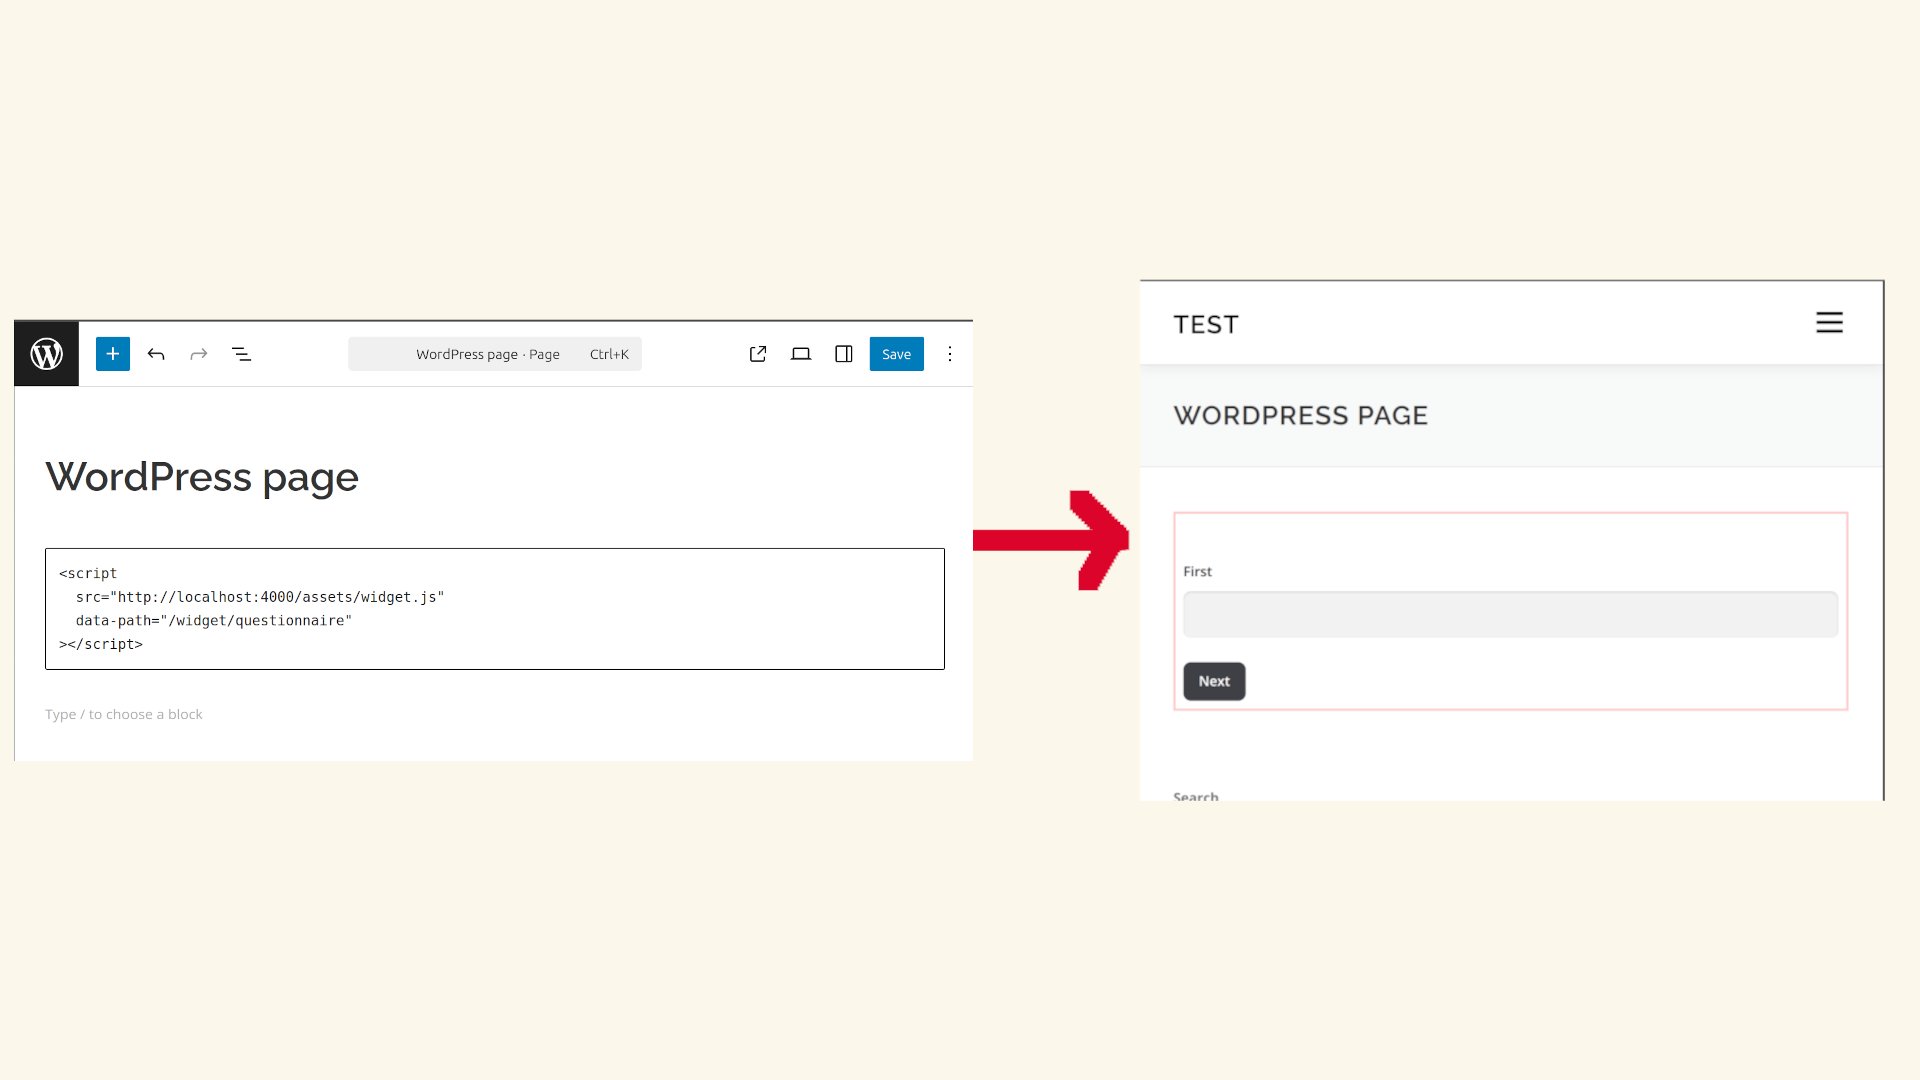
\includegraphics[width=1\linewidth]{images/goal.png}
\end{frame}

\begin{frame}{Steps needed to render a LiveView page}
  \begin{itemize}
    \item Load html though a normal http request.
    \item Mound LiveSocket through a js script.
  \end{itemize}
\end{frame}

\section{Methodology}

\begin{frame}{Fetch html}

  \begin{itemize}
    \item Fetch html.
    \item Create container.
    \item Add fetched html as innerHtml to the container.
    \item Attach container above script.
  \end{itemize}
  \centering
  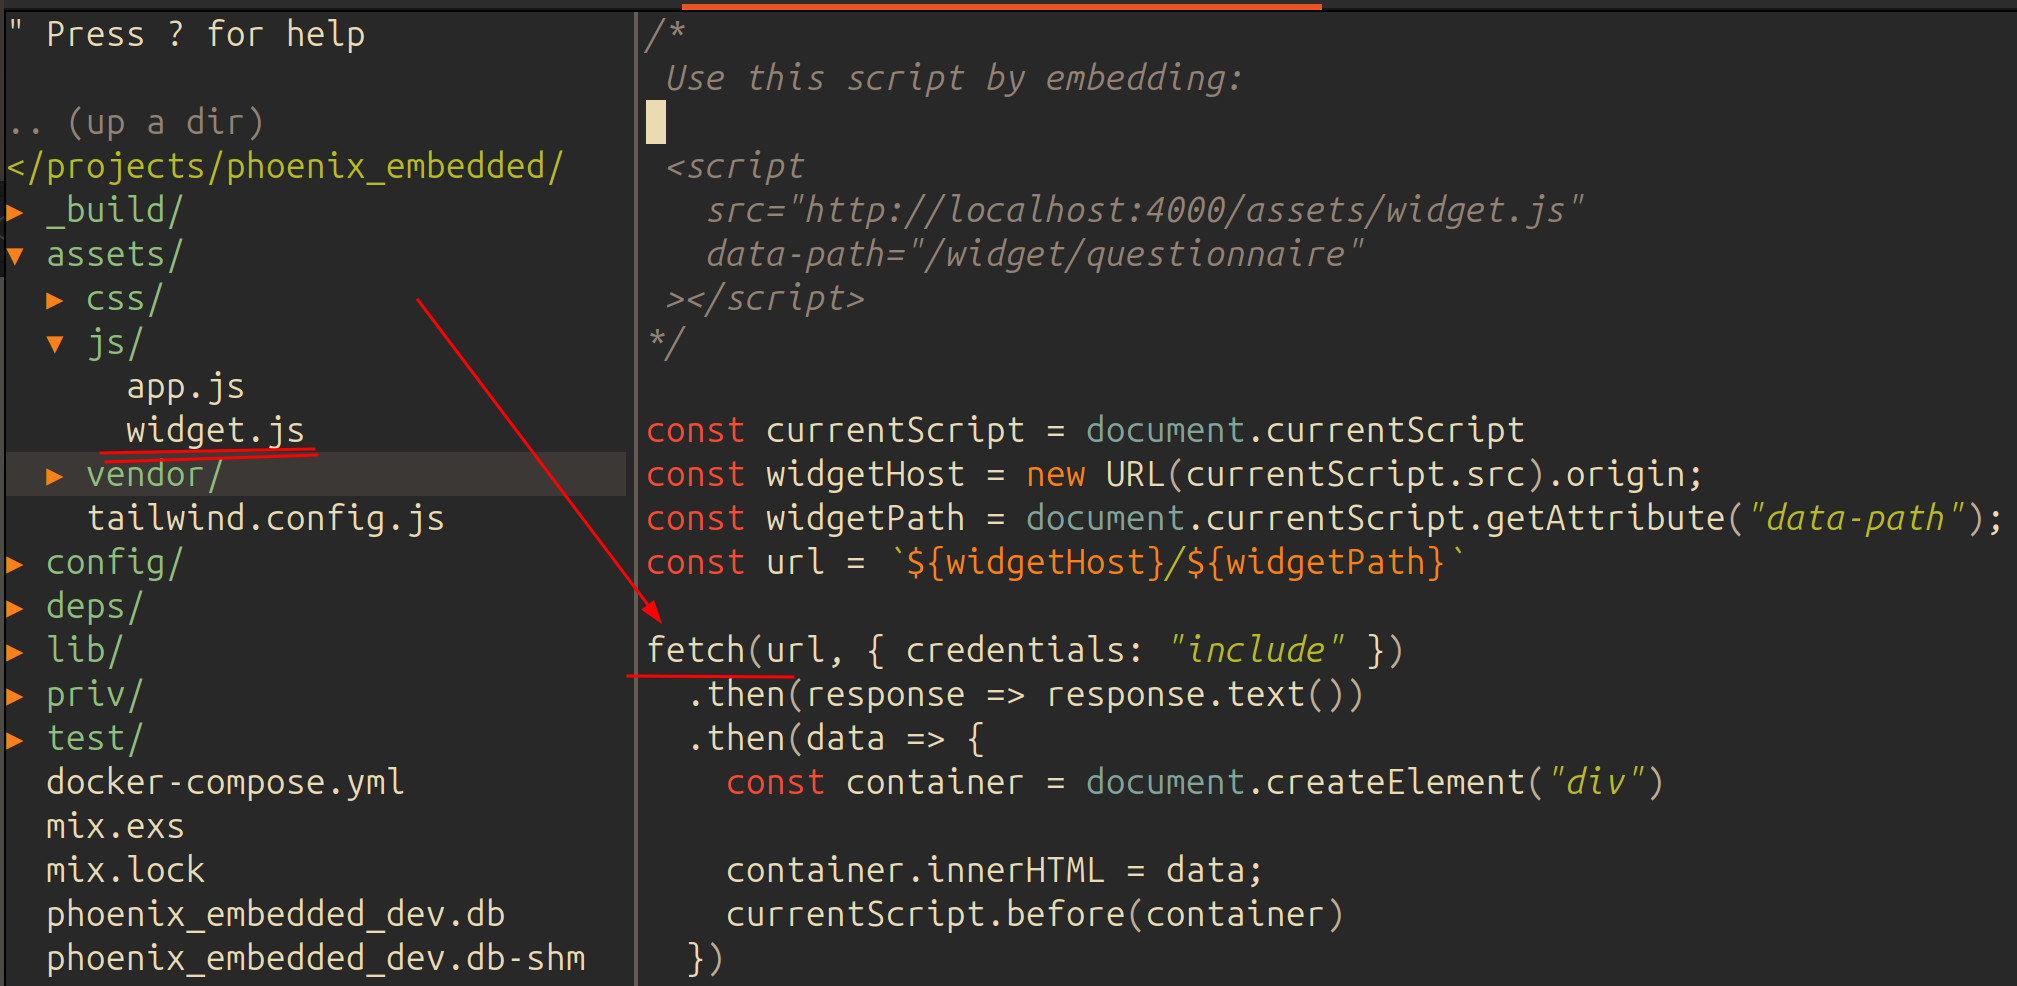
\includegraphics[width=0.8\linewidth]{images/fetch-html.png}
\end{frame}

\begin{frame}{Fix cors error}
  \centering
  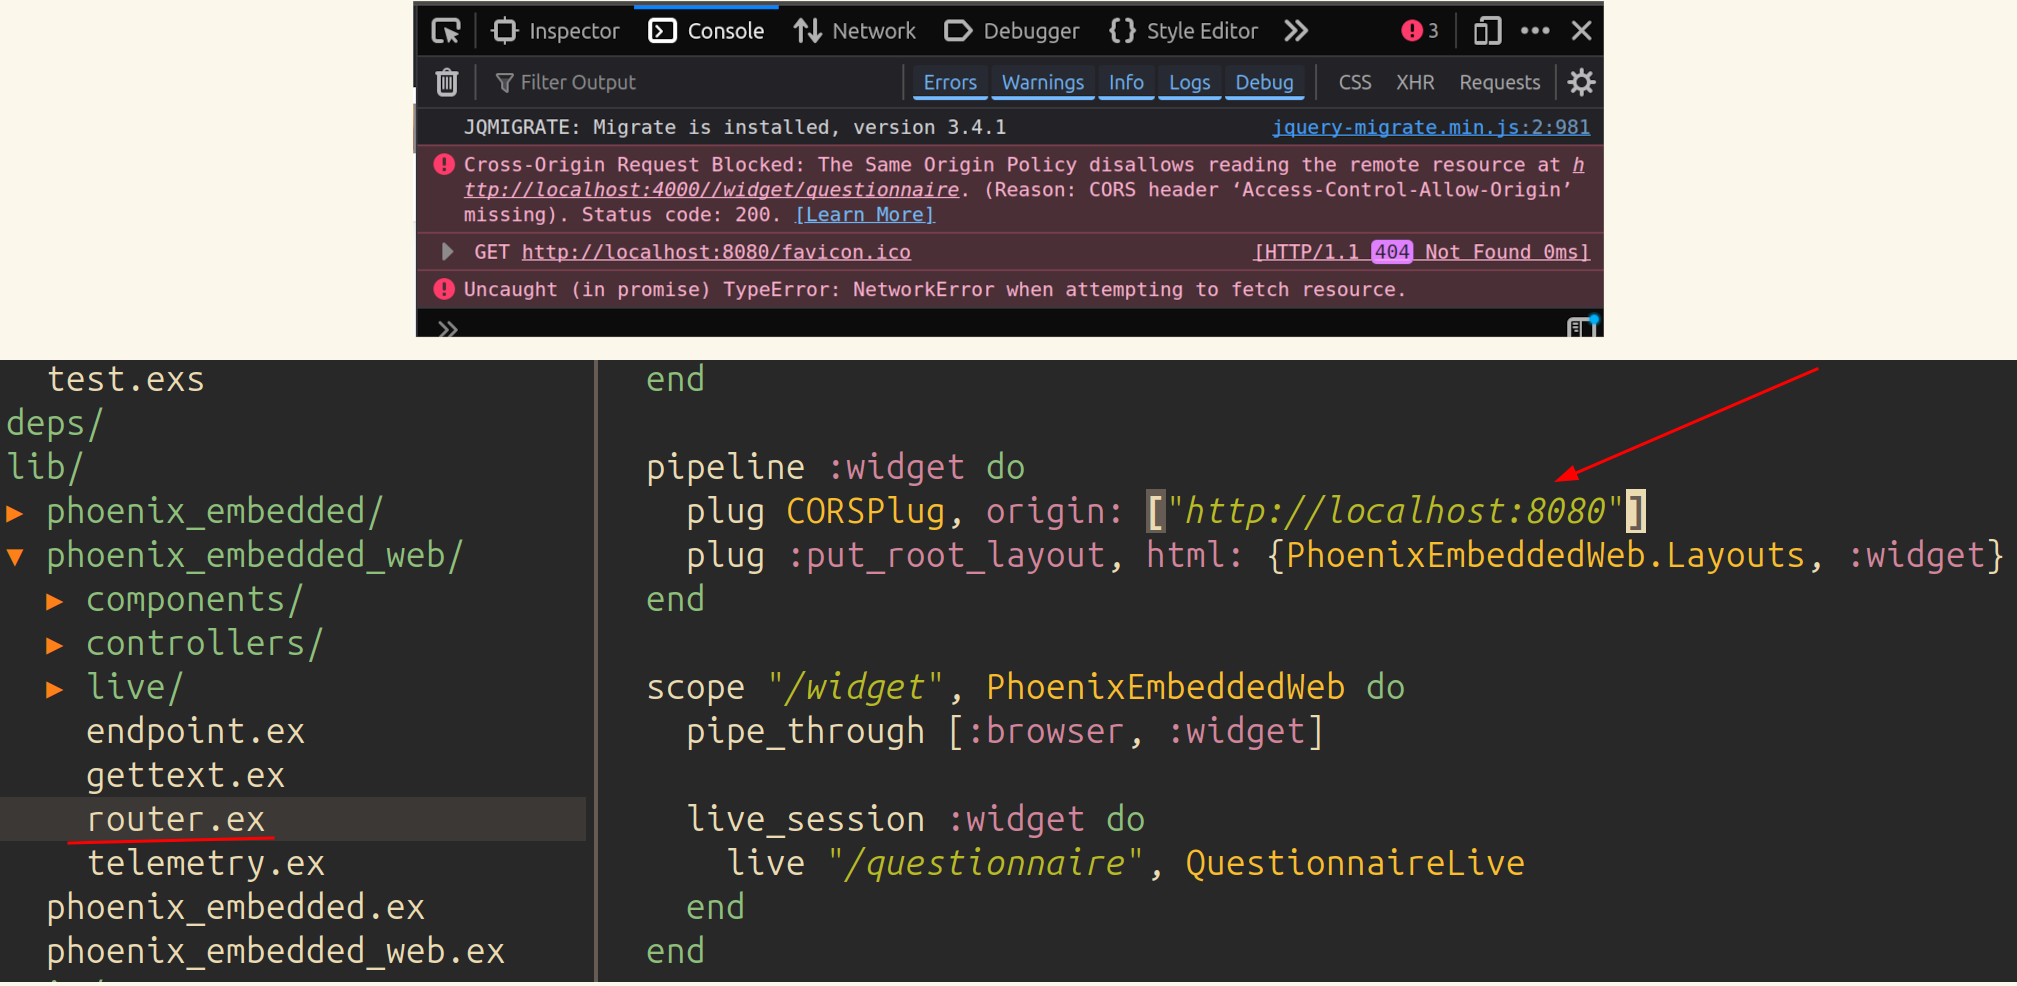
\includegraphics[width=0.8\linewidth]{images/cors.png}
\end{frame}

\begin{frame}{Use separate layout}
\begin{itemize}
  \item Layout without header or body.
  \item Without LiveView layout.
  \item With stylesheet link.
\end{itemize}
\centering
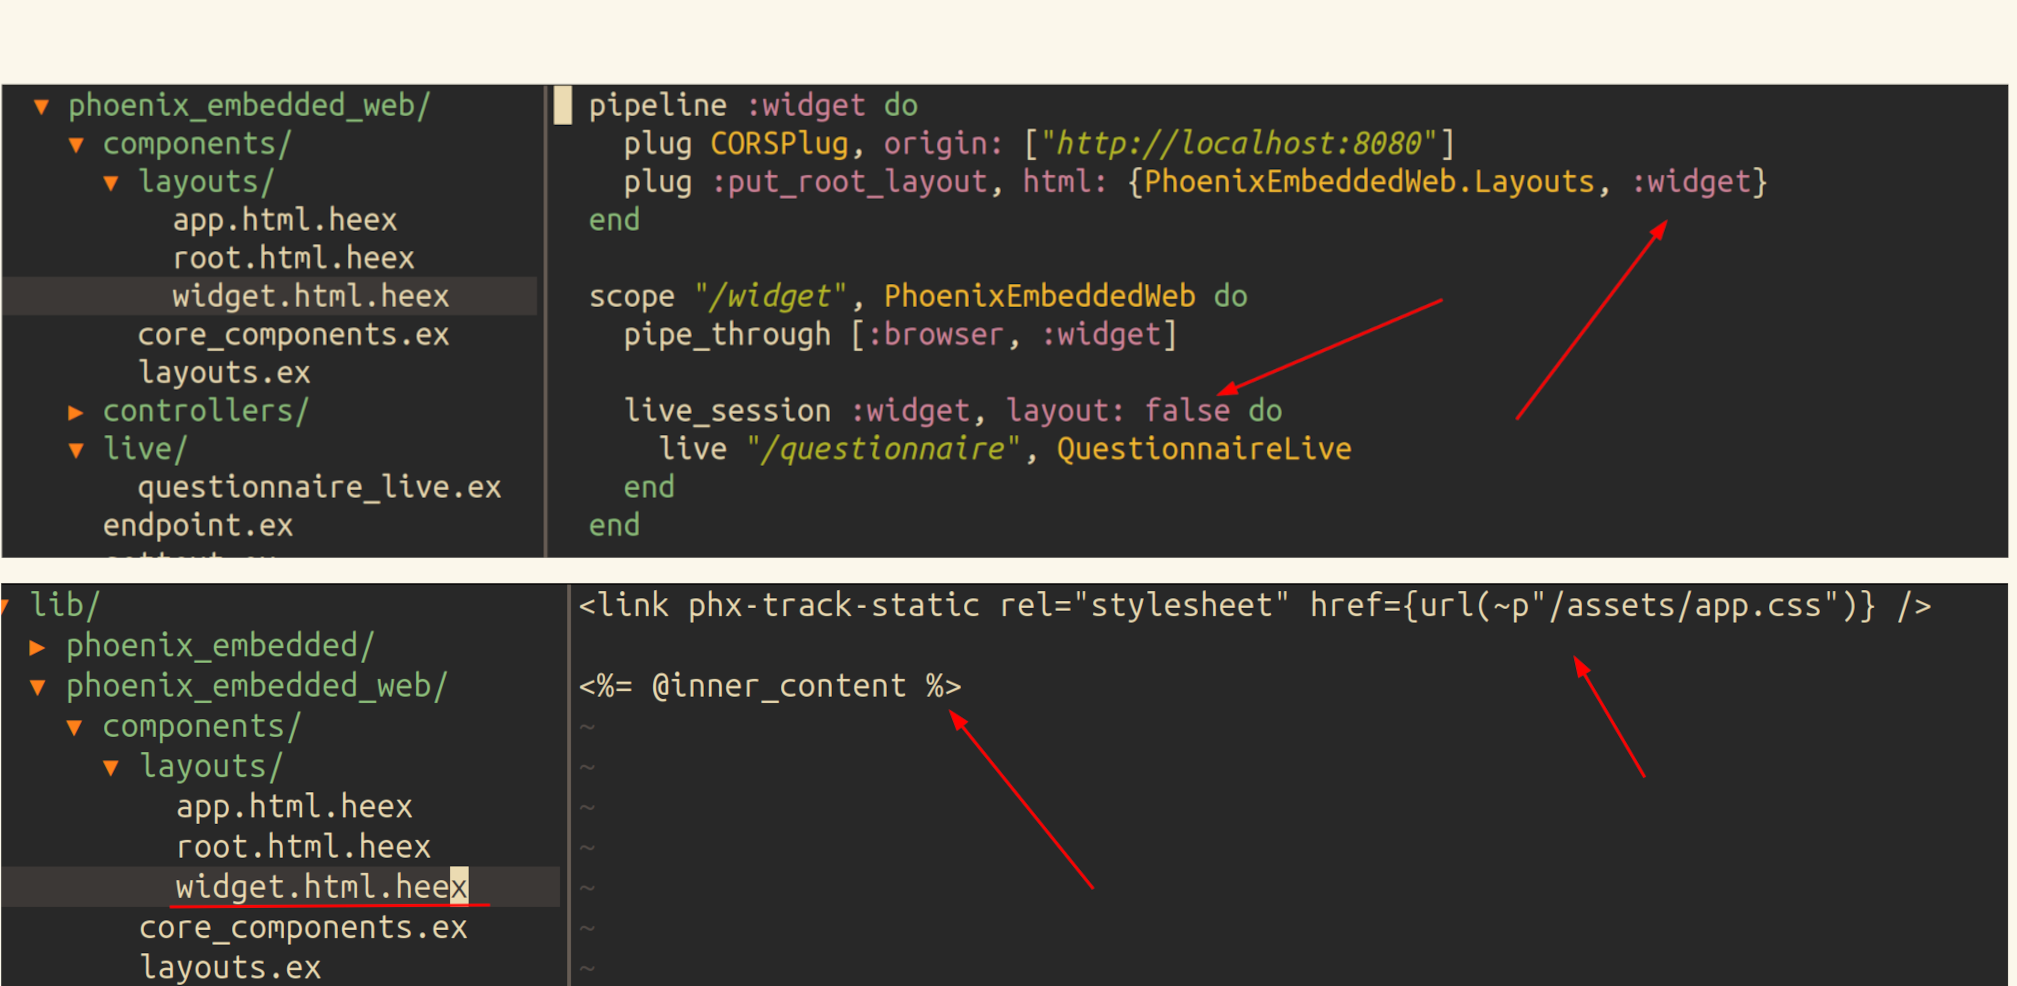
\includegraphics[width=0.8\linewidth]{images/layout.png}
\end{frame}

\begin{frame}{Mount LiveSocket}
\begin{itemize}
  \item Copy LiveSocket code from app.js.
  \item Add csrf token to layout.
\end{itemize}
\centering
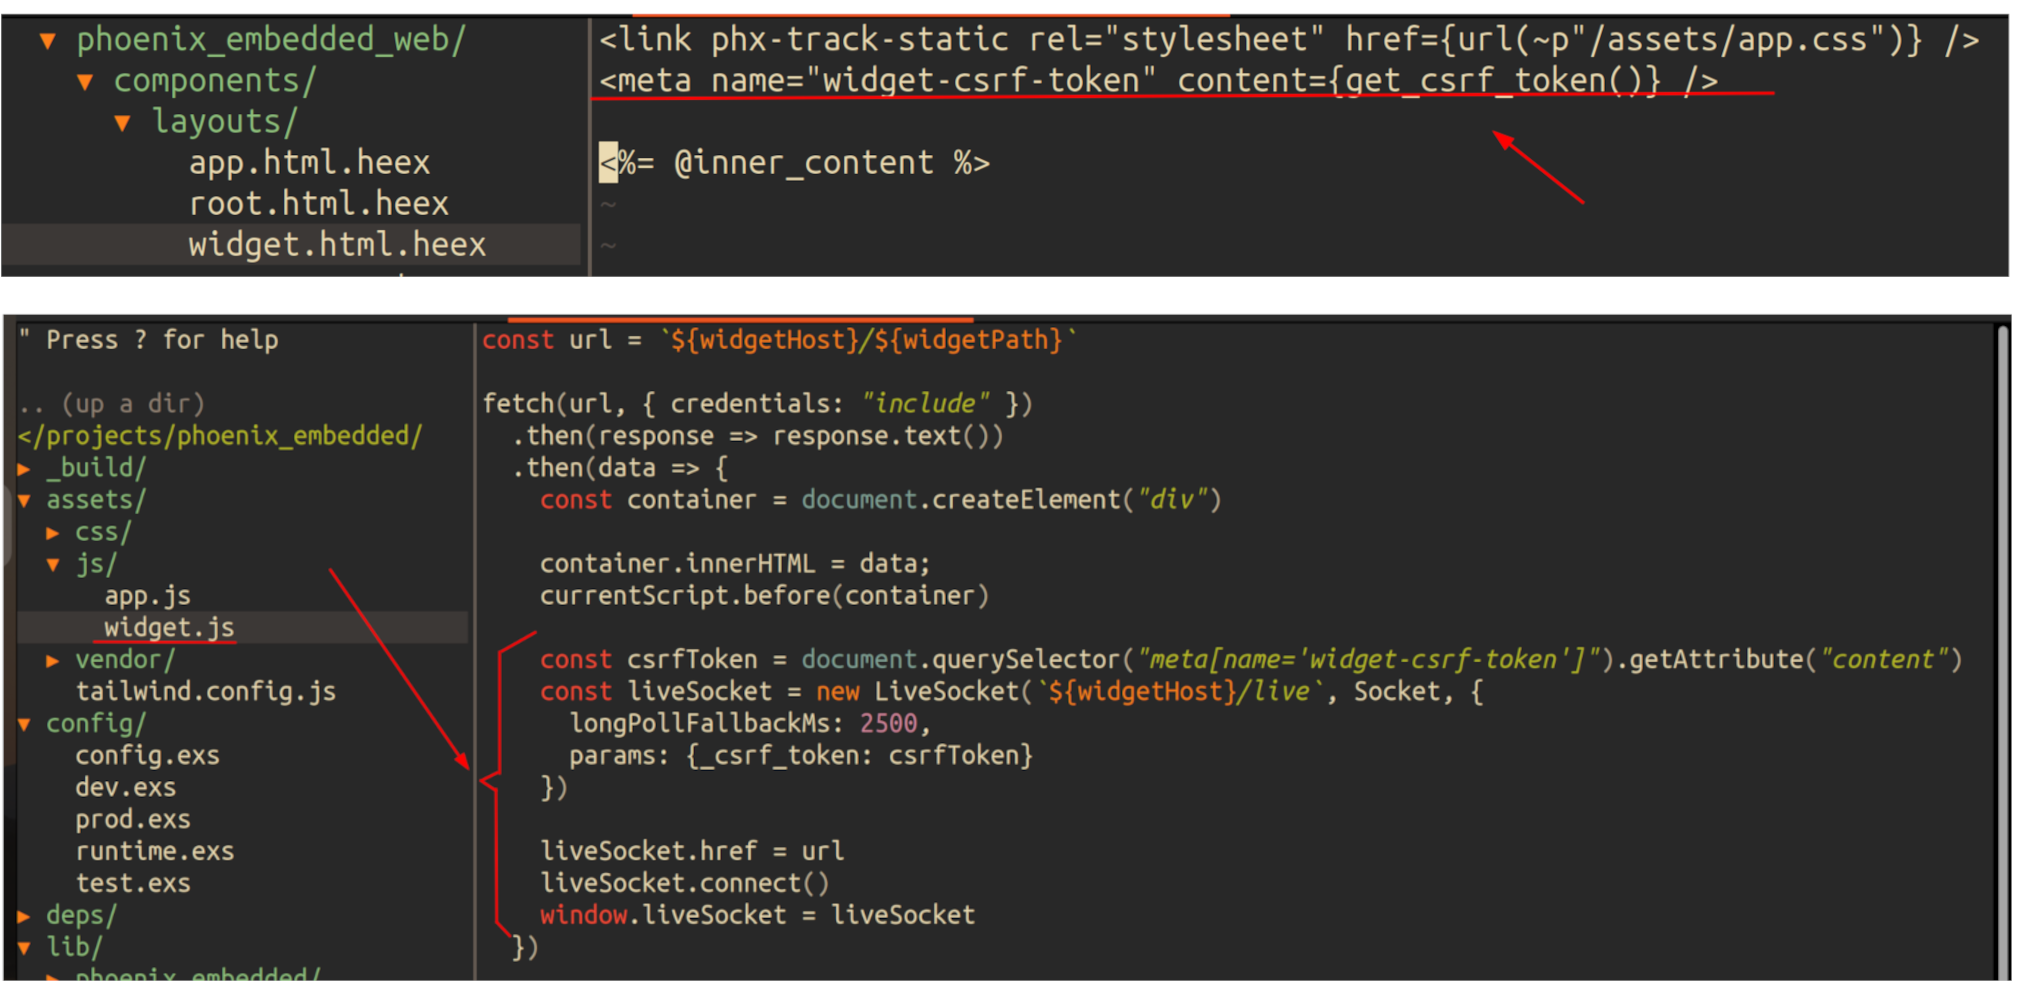
\includegraphics[width=0.8\linewidth]{images/mount-socket.png}
\end{frame}

\begin{frame}{Multi step form}
\begin{itemize}
  \item Use one LiveView page.
  \item Hide/show parts when one clicks on next.
  \item Use global form to make reconnection work correctly.
  \item Use hidden fields for internal assigns.
\end{itemize}
\centering
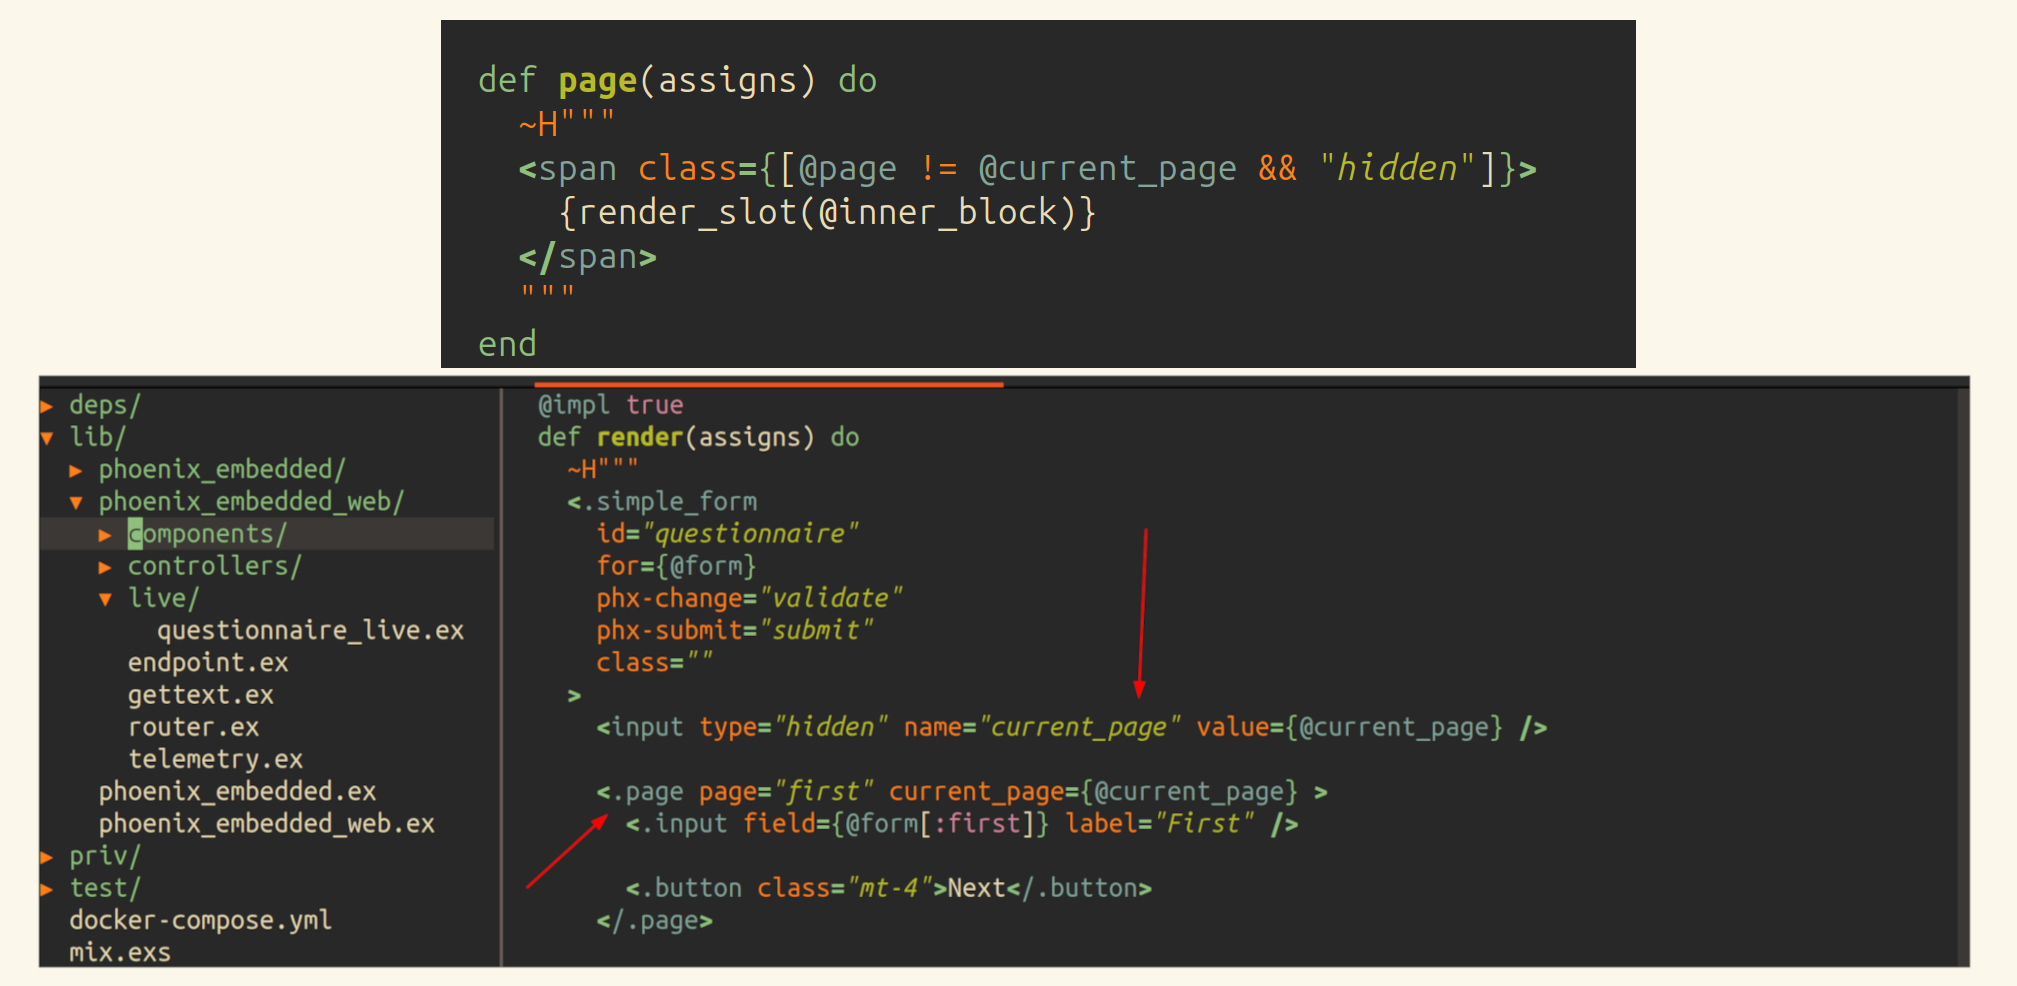
\includegraphics[width=0.8\linewidth]{images/multi-step-form.png}
\end{frame}

\section{Results}

\begin{frame}{Demo}
  \centering
  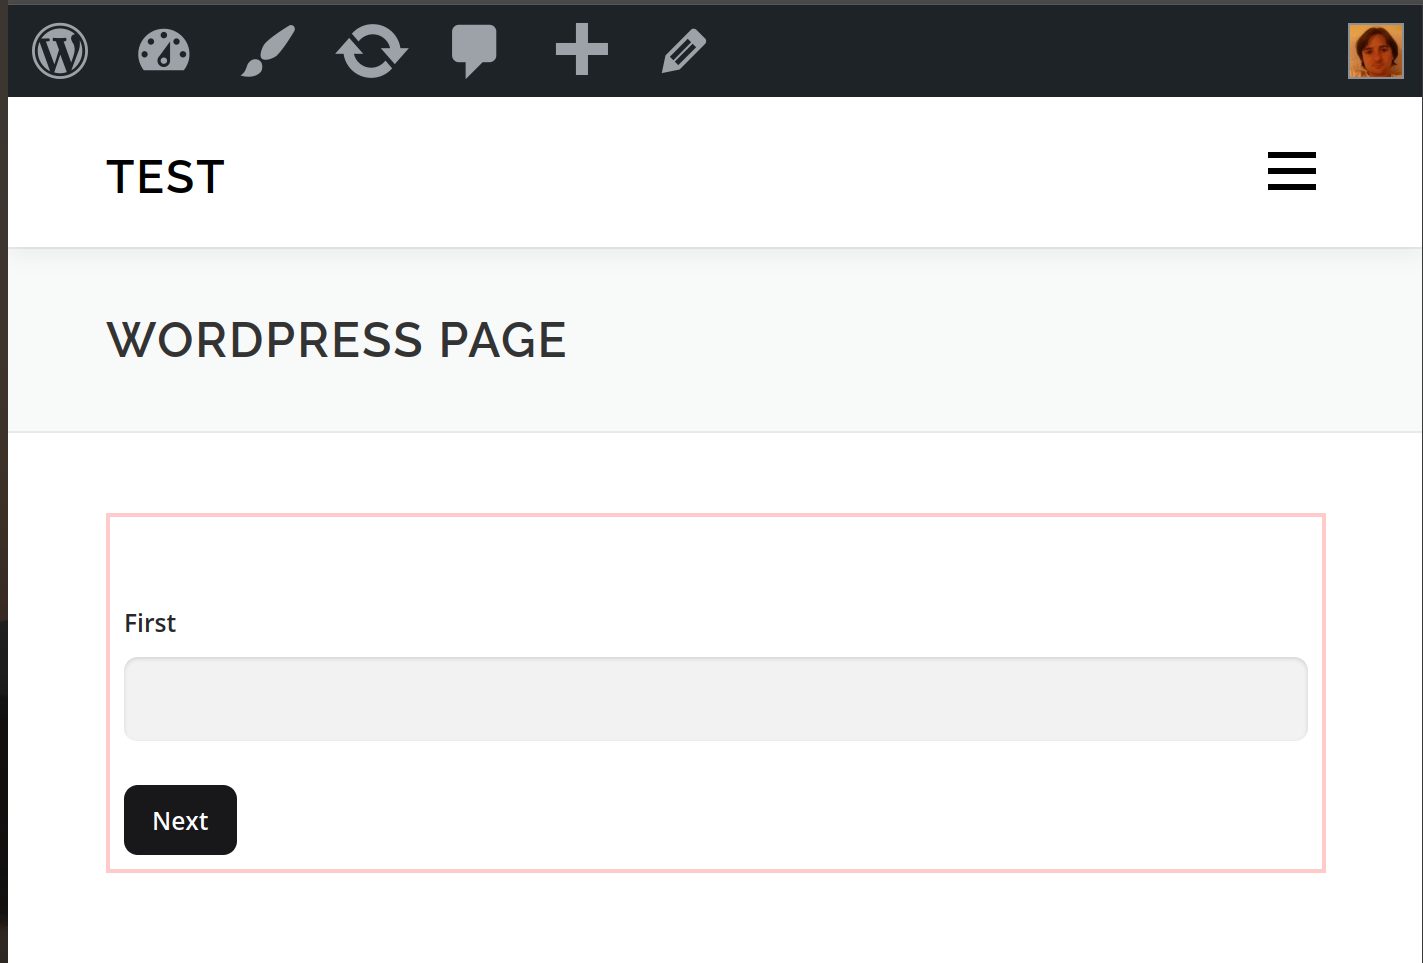
\includegraphics[width=1\linewidth]{images/demo.png}
\end{frame}

\begin{frame}[containsverbatim]{Debug}
\begin{itemize}
  \item Open external page.
  \item Open console.
  \item Paste something like the following in the console.
\end{itemize}
\hfill \break
\centering
\begin{minted}{javascript}
// remove current page content
main = document.querySelectorAll("main")[0]
new_main = document.createElement("main")
main.replaceWith(new_main)

// load LiveView page
script = document.createElement("script")
script.src = "http://localhost:4000/assets/widget.js"
script.setAttribute("data-path", "/widget/questionnaire")
new_main.appendChild(script)
\end{minted}
\end{frame}


\begin{frame}{Thank You!}
  \centering
  \Large Questions? \\
  \vspace{1cm}
  \normalsize
  \href{your.email@example.com}{aronwolf90@gmail.com}
\end{frame}

\end{document}
